\section{Simulador}

	En este capítulo se presenta un simulador basado en las ecuaciones de movimiento del boomerang obtenidas en el capítulo anterior, las cuales se muestran a continuación:

		\begin{equation}
		\begin{matrix}
		\dot{\omega}_{z}=\frac{T_{y}}{{I}_{3}}\\
		\dot{V}=\frac{1}{m}(-{F}_{x}\cos{\Psi}-{F}_{z}\sin{\Psi})\\
		\dot{\Psi}=\frac{1}{m }({F}_{x}\sin{\Psi-{F}_{z}\cos{\Psi}})+\frac{{T}_{x}}{{I}_{3}{\omega}_{z}} \\
		\end{matrix}\\
		\label{ec61}
		\end{equation}

		\begin{equation}
		\begin{matrix}
		 {\dot{\vartheta}}=\frac{1}{{I}_{3}{\omega}_{z}}(-{T}_{y}\cos{\eta}-{T}_{x}\sin{\eta})\\
		 \dot{\varphi}=\frac{1}{{I}_{3}{\omega}_{z}}\frac{1}{\sin{\vartheta}}(-{T}_{y}\sin {\eta}+{T}_{x}\cos{\eta})\\
		 \dot{\eta}=-\frac{{F}_{y}}{mV\cos{\Psi}}-\tan{\Psi}\frac{T_{y}}{{I}_{3}{\omega}_{z}}-\dot{\varphi} \cos{\vartheta} \\
		\end{matrix}
		\label{ec62}
		\end{equation}

		\begin{equation}
		\begin{matrix}
		\dot{X} = V[{-\cos{\Psi}(\cos{\eta}\cos{\varphi}-\sin{\eta}\sin{\varphi}\cos{\vartheta})-\sin{\Psi}\sin{\varphi}\sin{\vartheta}]}\quad\\
	    \dot{Y}=V[{-\cos{\Psi}\left(\cos{\eta}\sin{\varphi}+\sin{\eta}\cos{\varphi}\cos{\vartheta}\right)+\sin{\Psi}\cos{\varphi}\sin{\vartheta}]}\\
	    \dot{Z}=V[{-\cos{\Psi\sin{\eta}\sin{\vartheta}-\sin{\Psi}\cos{\vartheta}}]}
		\end{matrix}
		\label{ec63}
		\end{equation}

	Para las fuerzas y pares aerodinámicos actuantes en el boomerang se tiene la siguiente ecuación:

		\begin{subequations}
    	\begin{align}
		{\vec{F}}_{a}={\mu}_{a}{a}^{4}{\omega}_{z}^{2}{\vec{F}}_{1}(\Psi,U)\\
		{\vec{T}}_{a}={\mu}_{a}{a}^{5}{\omega}_{z}^{2}{\vec{T}}_{1}(\Psi,U)
		\end{align}
		\label{ec64}
		\end{subequations}

	Las ecuaciones de movimiento del boomerang son ecuaciones diferenciales de primer orden las cuales pueden aproximarse por un método de integración y así poder reeconstruir la trayectoria de vuelo del boomerang en un tiempo determinado.

	\subsection{Regla de Simpson}

	Al ser de gran interés la posición del boomerang con respecto al sistema coordenado fijo es necesario resolver las ecuaciones de movimiento, para esto se propone utilizar el método de integración de Simpson.
	La regla de simpson es un método de integración numérica para obtener el valor aproximado de integrales definidas en un intervalo [a,b], mediante la regla del trapecio, es decir, que sobre cada subintervalo en el que se divide [a,b] se aproxima una función $f$ por un polinomio de primer grado, para luego calcular los trapecios formados en esos intervalos. Espefícificamente la aproximación se realiza de la siguiente manera\cite{Granville}:

		\begin{equation}
		\int_{a}^{b} f(x)dx \approx \frac{b-a}{6} \left[ f(a) + 2f(a) + 2f(b) + f(b)\right]
		\label{ec65}
		\end{equation}

	Cada una de las ecuaciones de movimiento del boomerang se integran con esta regla, para lo cual se toma en cuenta que se integran con respecto al tiempo y se obtiene la aproximación en un intervalo de tiempo.

	\subsection{Algoritmo de la simulación}

	Se comienza definiendo el intervalo de tiempo [a,b] en donde se emplea la aproximación, el cual será representado por un diferencial de tiempo $(dt)$.

	Se establecen las condiciones iniciales necesarias para realizar el cálculo, las cuales se enlistan a continuación:

		\begin{enumerate}
		\item{g = aceleración de la gravedad {($\frac{m}{seg}$)}.}
		\item{$my$ = densidad del aire .}
		\item{m = masa del boomeang {($g$)}.}
		\item{I3 = momento de inercia del boomerang {($\frac{g}{dm^{2}}$)}.}
		\item{r = radio del centro de masa a cada una de las aspas del boomerang {($mm$)}.}
		\item{vel$\_$v = velocidad del viento {($\frac{m}{seg}$)}.}
		\item{vel$\_$ini = Velocidad inical {($\frac{m}{seg}$)}.}
		\item{ang$\_$v = ángulo del viento {($\frac{m}{seg}$)}.}
  		\item{ang$\_$lanzamiento = ángulo del lanzamiento del boomerang {($\frac{m}{seg}$)}.}
		\item{giro = velocidad angular inicial{($Hz$)}.}
		\item{dt = período de integración.}
     	\item{X = Posición Inicial en X $m$.}
     	\item{Y = Posición Inicial en Y $m$.}
     	\item{Z = Posición Inicial en Z $m$.}
		\end{enumerate}

	Se toma en cuenta un valor aproximado de la aceleración de la gravedad y de la densidad del aire, además se fija un período de integración:

		\begin{enumerate}
		\item{g = 9.81 {($\frac{m}{seg}$)}.}
		\item{$my$ = 1.2 ($\frac{kg}{m^{3}}$).}
		\item{dt = 0.1 $seg$.}
		\end{enumerate}

	Para el boomerang construido para el desarrollo de este proyecto, se tiene lo siguiente:

		\begin{enumerate}
		\item{m = 230 {($g$)}.}
		\item{I3 = 478 {($\frac{g}{dm^{2}}$)}.}
		\item{r = 250 {($mm$)}.}
		\end{enumerate}


	Las demás condiciones iniciales del vuelo pueden variar entre simulaciones para realizar pruebas al modelo.

	Utilizando la regla de simpson y con las condiciones iniciales se muestra el la Fig. (\ref{fig14}) diagrama de flujo donde se detalla el algoritmo para el cálculo de la trayectoria de vuelo del boomerang.

		\begin{figure}[h]
		\begin{center}
		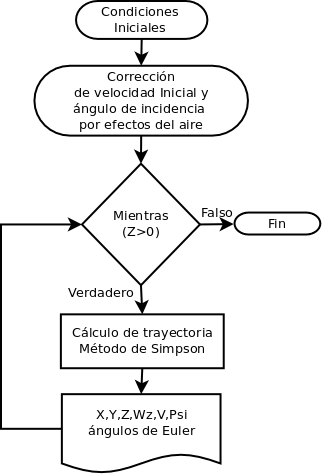
\includegraphics[scale=0.4]{imagenes/3-boomerang/diag_flu_tra.png}
		\caption{Algoritmo de cálculo de la trayectoria de vuelo del boomerang.}
		\label{fig14}
		\end{center}
		\end{figure}

\newpage
	\subsection{Interfaz de la simulación}


	El simulador de la trayectoria de vuelo del boomerang se realiza en la Interfaz Gráfica de Usuario (GUI por sus siglas en ingles) que provee $Matlab_{\textregistered}$. En la Fig. (\ref{fig15}) se muestra la intefaz gráfica creada para asignar los parámetros iniciales y observar la gráfica generada por el vuelo del boomerang.

		\begin{figure}[h]
		\begin{center}
		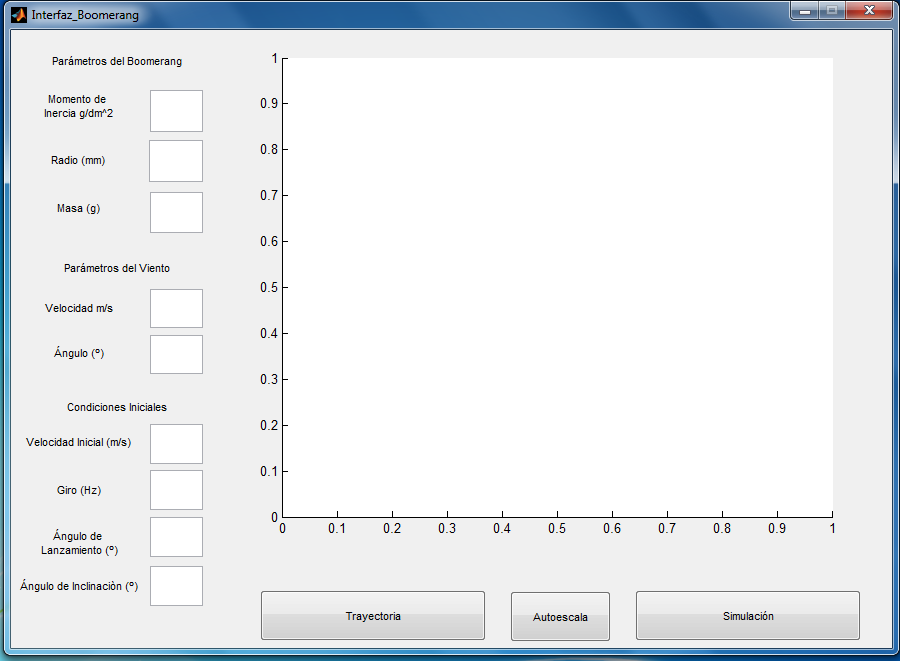
\includegraphics[scale=0.4]{imagenes/3-boomerang/GUIDE.png}
		\caption{Interfaz gráfica en la GUI de Matlab.}
		\label{fig15}
		\end{center}
		\end{figure}

\newpage
    \subsection{Simulaciones del modelo}

    Para la primer prueba del modelo se establecen los siguientes parámetros de vuelo iniciales:

		\begin{enumerate}
		\item{vel$\_$v = 0 {($\frac{m}{seg}$)}.}
		\item{vel$\_$ini = 31 {($\frac{m}{seg}$)}.}
		\item{ang$\_$v = 0 {($grados$)}.}
  		\item{ang$\_$lanzamiento $\approx$ 30 {($grados$)}.}
		\item{giro $\approx$ 10 {($Hz$)}.}
     	\item{X = 0 $m$.}
     	\item{Y = 0 $m$.}
     	\item{Z = 1.8 $m$.}
		\end{enumerate}

	En la Fig. \ref{fig16} se muestra el resultado generado por la simulación con los datos iniciales propuestos:

		\begin{figure}[h]
		\begin{center}
		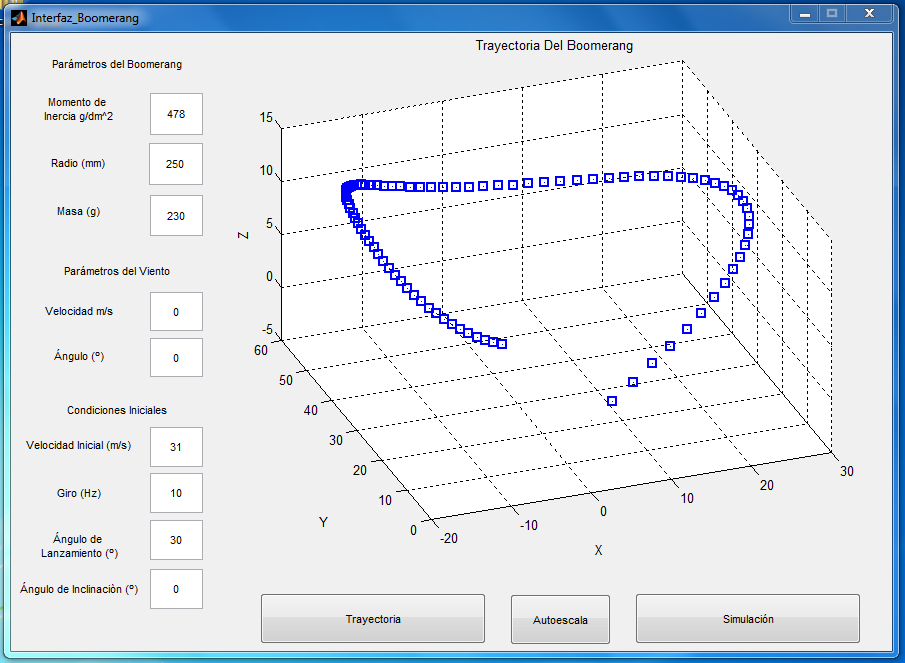
\includegraphics[scale=0.45]{imagenes/3-boomerang/tray_1.png}
		\caption{Simulación 1 del modelo.}
		\label{fig16}
		\end{center}
		\end{figure}


	En la segunda prueba del modelo se agrega velocidad y ángulo de la velocidad del viento actuante en el boomerang:

		\begin{enumerate}
		\item{vel$\_$v = 5 {($\frac{m}{seg}$)}.}
		\item{vel$\_$ini = 26 {($\frac{m}{seg}$)}.}
		\item{ang$\_$v = 20 {($grados$)}.}
  		\item{ang$\_$lanzamiento $\approx$ 20 {($grados$)}.}
		\item{giro $\approx$ 10 {($Hz$)}.}
     	\item{X = 0 $m$.}
     	\item{Y = 0 $m$.}
     	\item{Z = 1.8 $m$.}
		\end{enumerate}

	De igual manera en la Fig. \ref{fig17} se muestra la trayectoria de vuelo del boomerang generada por los datos iniciales propuestos:

		\begin{figure}[h]
		\begin{center}
		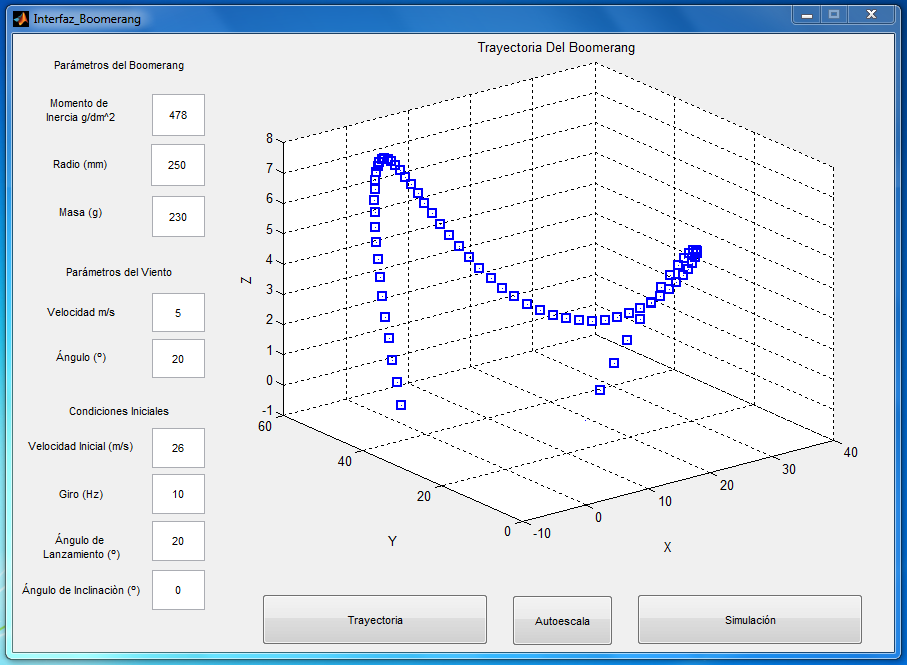
\includegraphics[scale=0.45]{imagenes/3-boomerang/tray_2.png}
		\caption{Simulación 2 del modelo.}
		\label{fig17}
		\end{center}
		\end{figure}

	Finalmente se muestra una simulación con baja velocidad angular y un valor grande del ángulo de lanzamiento:

		\begin{enumerate}
		\item{vel$\_$v = 0 {($\frac{m}{seg}$)}.}
		\item{vel$\_$ini = 15 {($\frac{m}{seg}$)}.}
		\item{ang$\_$v = 0 {($grados$)}.}
  		\item{ang$\_$lanzamiento $\approx$ 60 {($grados$)}.}
		\item{giro $\approx$ 10 {($Hz$)}.}
     	\item{X = 0 $m$.}
     	\item{Y = 0 $m$.}
     	\item{Z = 1.8 $m$.}
		\end{enumerate}

	En la Fig. \ref{fig18} se muestra la trayectoria de vuelo del boomerang generada por los datos iniciales propuestos:

		\begin{figure}[h]
		\begin{center}
		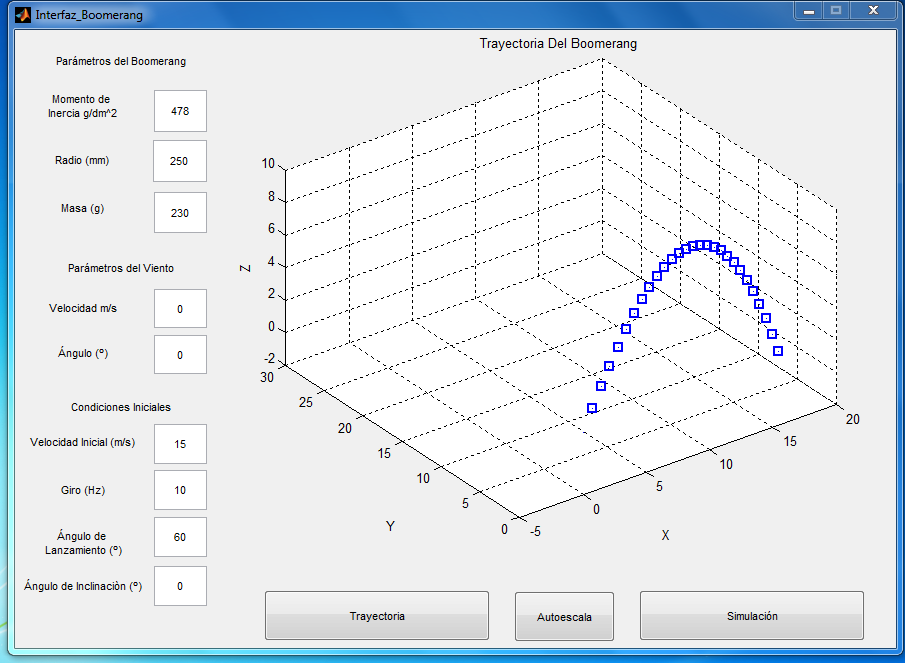
\includegraphics[scale=0.45]{imagenes/3-boomerang/tray_3.png}
		\caption{Simulación 3 del modelo.}
		\label{fig18}
		\end{center}
		\end{figure}

\newpage
	Como es posible observar en la Fig. (\ref{fig16}) y en la Fig.(\ref{fig16}), al aplicarle una velocidad grande al boomerang, con ó sin velocidad del viento, el boomerang tiende a regresar cerca del punto de lanzamiento, esto debido a que los efectos presentes en el boomerang se mantienen durante el vuelo.

	En cambio en la Fig. (\ref{fig18}), el boomerang no regresa al punto de lanzamiento debido a la baja velocidad inicial con la que el boomerang fué lanzado.

	Por lo que la simulación resulta ser una aproximación a la trayectoria que genera un vuelo del boomerang.
